\documentclass[aspectratio=169,10pt,dvipsnames]{beamer}

\setbeameroption{show notes}

\input{preamble.inc}

\newcommand{\myfbox}[2]{\tikz[baseline=(n.base)]\node(n)[alt=<1>{fill=#1!50}]{#2};}

\title{La struttura delle proposizioni semplici}

\begin{document}

\begin{frame}
\titlepage
\end{frame}

\begin{frame}{Inferenze a livello predicativo}
    Fino ad ora abbiamo trattato la \emph{logica proposizionale}. Nella logica proposizionale il costrutto di base è la proposizione, e proposizioni più complesse si ottengono tramite connettivi logici.

    \medskip
    Quando entrano in gioco i \emph{quantificatori}, la logica proposizionale non è più sufficiente per determinare la validità di una inferenza.

    \begin{center}
        \begin{inference}
            Napoleone è corso\\
            Tutti i corsi sono francesi\\
            \hline
            Napoleone è francese
        \end{inference}
        \qquad
        \begin{inference}
            Socrate è un uomo\\
            Tutti gli uomini sono mortali\\
            \hline
            Socrate è mortale
        \end{inference}
    \end{center}
    Se analizzate come fatto fin'ora, corrispondo alla regola di inferenza:
    \begin{center}
        \begin{inference}
            A\\
            B\\
            \hline
            C
        \end{inference}
    \end{center}
    che non è corretta! Bisogna passare alla \alert{logica dei predicati} e iniziare ad indagare la \alert{struttura delle proposizioni semplici}.
\end{frame}

\section{Proposizioni semplici del 1° tipo}

\begin{frame}{Proposizioni semplici del primo tipo}
	Consideriamo queste proposizioni semplici:
	\begin{center}
		\itshape
		Stefano {\only<2->{\color{brown}}è italiano}\\
		Marco {\only<2->{\color{brown}}sta leggendo}\\
		Carlo {\only<3->{\color{green}}è più alto di} Massimo\\
		Monza {\only<3->{\color{green}}ha più abitanti} di Milano\\
		Dario {\only<4->{\color{blue}}è figlio di} Ernesto {\only<4->{\color{blue}}e} Maria\\
		Marcello {\only<4->{\color{blue}}va a} Torino {\only<4->{\color{blue}}con}  Claudia
	\end{center}
	In queste proposizioni interviene:
	\begin{itemize}
		\item<2-> una \textcolor{brown}{proprietà} \tikz[remember picture] \node (i1) {};
		\item<3-> una \textcolor{green}{relazione binaria} \tikz[remember picture] \node (i2) {};
		\item<4-> una \textcolor{blue}{relazione ternaria} \tikz[remember picture] \node (i3) {};
		\item<5-> in generale, una relazione $n$-aria \tikz[remember picture] \node (i4) {};
	\end{itemize}
	\visible<7->{
		\begin{definition}[Proposizioni semplici del primo tipo]
		Le \alert{proposizioni semplici del primo tipo} sono proposizioni in cui un predicato ad $n$ argomenti viene applicato ad $n$ individui.
	\end{definition}
	}
	\visible<6->{\begin{tikzpicture}[remember picture, overlay]
		\node (p) [right=4cm of i2] {\alert{predicati}};
		\draw [->,red] (i1) edge (p);
		\draw [->,red] (i2) edge (p);
		\draw [->,red] (i3) edge (p);
		\draw [->,red] (i4) edge (p);
	\end{tikzpicture}}
\end{frame}

\note{Valutare se eliminare completamente il concetto di tipo di una proposizione semplice.}

\begin{frame}{Individui e termini}
	Cosa sia un individuo dipende dal contesto: persone, numeri, pianeti, etc\ldots

	\pause\medskip
	Ci si può riferire ad un individuo in vari modi:
	\begin{itemize}
		\item tramite un \alert{nome} proprio: Carlo, 13, Giove
		\item tramite una \alert{descrizione definita} che comunque lo identifica in maniera univoca: il fratello di Michele, 15-2, il pianeta più grande del sistema solare
	\end{itemize}
	\begin{example}[Proposizioni con descrizioni definite]
		\centering
		\itshape
		\alert{Il cane di Giovanni} è fedele\\
		\alert{Il figlio di Aldo} ha sposato \alert{la sorella di Giuseppe}\\
		\alert{$5^2+3$} è pari
	\end{example}
	\pause
	In logica, nomi e descrizioni definite sono anche chiamati \alert{termini}.
\end{frame}

\section{Proposizioni semplici del 2° tipo}

\begin{frame}{Quantificatori}
	Consideriamo queste proposizioni semplici:
	\begin{center}
		\itshape
		Tutti gli uomini sono mortali\\
		Vi è un italiano più alto di due metri\\
		Ogni studente universitario frequenta almeno un corso
	\end{center}
	Contengono dei \alert{quantificatori}: \emph{tutti}, \emph{ogni}, \emph{vi è}, \emph{almeno}.

	\pause
	\medskip
	Prenderemo in considerazione soltanto due quantificatori:
	\begin{itemize}
		\item \alert{per ogni}, chiamato \alert{quantificatore universale}, che equivale a \emph{tutti}, \emph{ogni}, etc..\\[0.1cm]
		``\emph{per ogni $x$, \ldots}'' significa: tutti gli individui soddisfano \ldots
		\item \alert{esiste}, chiamato \alert{quantificatore esistenziale}, che equivale a \emph{vi è}, \emph{almeno}, etc..\\[0.1cm]
		``\emph{esiste x tale che \ldots}'' significa: vi è almeno un individuo che soddisfa \ldots
	\end{itemize}

	\medskip
	L'uso di questi due quantificatori richiede l'introduzione di lettere come $x$, $y$, $z$, \ldots, chiamate \alert{variabili individuali}.
\end{frame}

\note{TODO. Propongo di cambiare l'ordine in cui si presentano gli argomenti: prima introdurre le funzioni proposizionali, poi i quantificatori per ogni ed esiste, poi le variabili libere e vincolate, infine i quantificatori del linguaggio naturale.

\medskip Con i quantificatori del linguaggio naturale, focalizzarsi sul fatto che essi eliminano le variabili rimpiazzandoli con pronomi indefiniti

\medskip Valuate inoltre se spostare tutta questa cosa dei quatificatori quando si introdurrà la logica dei predicati.}

\begin{frame}{Per ogni ed esiste (1)}
	La maggior parte dei quantificatori possono essere riscritti usando solo \emph{per ogni} ed \emph{esiste}.

	\begin{example}[Usare i quantificatori per ogni ed esiste]
		\centering\itshape
		Tutti gli uomini sono mortali\\
		$\Downarrow$\\
		Per ogni $x$, se $x$ è un uomo, allora $x$ è mortale.\\
		\medskip
		\pause
		Vi è un italiano più alto di due metri\\
		$\Downarrow$\\
		Esiste $x$ tale che $x$ è italiano ed $x$ è alto più di due metri.\\
		\medskip
	\pause
		Ogni studente universitario frequenta almeno un corso\\
		$\Downarrow$\\
		Per ogni $x$, se $x$ è uno studente universitario, allora esiste $y$ tale che $y$ è un corso ed $x$ frequenta $y$
	\end{example}
\end{frame}

\begin{frame}{Per ogni ed esiste (2)}
	L'uso dei quantificatori \emph{per ogni} ed \emph{esiste} rende esplicita la forma logica di varie proposizioni del linguaggio naturale.

	\begin{example}[Esempio]
		La proposizione

		{\medskip \itshape
		\quad Per ogni $x$, se $x$ è un uomo, allora $x$ è mortale.
		}

		\medskip
		corrisponde a
		\begin{itemize}
			\item Tutti gli uomini sono mortali
			\item Gli uomini sono mortali
			\item Ogni uomo è mortale
			\item Qualunque uomo è mortale
			\item Ciascun uomo è mortale
			\item L'uomo è mortale
		\end{itemize}
	\end{example}
\end{frame}

\begin{frame}{Quantificatori vaghi e ambigui}
	Alcune osservazioni.
	\begin{enumerate}
		\item Nella lingua comune vi sono alcuni quantificatori \alert{vaghi} di cui non ci occupiamo:

		\medskip
		\begin{center}
			\itshape
			\textcolor{blue}{Quasi tutti} gli italiani sanno chi è il presidente della Repubblica.\\
			\textcolor{blue}{La maggior parte dei} nordici ha i capelli biondi.
		\end{center}
		\medskip\pause

		\item Alcuni quantificatori nella lingua italiana sono \alert{ambigui}.	Ad esempio:

		\medskip
		\begin{center}
			\itshape
			Se \textcolor{orange}{qualcuno} è buono, allora \textcolor{blue}{qualcuno} lo ama.\\
			$\Downarrow$\\
			\pause
			\textcolor{orange}{Per ogni $x$}, se $x$ è buono \textcolor{blue}{esiste $y$} tale che $y$ ama $x$.
		\end{center}
		\medskip

		La stessa parola ``\emph{qualcuno}'' gioca  due ruoli differenti da quantificatore esistenziale ed universale.
	\end{enumerate}
\end{frame}

\begin{frame}{Proposizioni semplici del secondo tipo}
	\begin{definition}
		Le proposizioni semplici che iniziano con ``\emph{per ogni}'' si dicono \alert{quantificate universalmente}, quelle che iniziano con ``\emph{esiste}'' si dicono \alert{quantificate esistenzialmente}.
	\end{definition}
	\begin{definition}[Proposizioni semplici del secondo tipo]
		Le \alert{proposizioni semplici del secondo tipo} sono le proposizioni quantificate universalmente o esistenzialmente.
\end{definition}
\end{frame}

\note{Esercizio 1.5, 1.4, 1.7}

\section{Variabili libere e vincolate}

\begin{frame}{Funzioni proposizionali e variabili libere}
	Analizziamo la proposizione ``{\itshape Per ogni $x$, se $x$ è un uomo, allora $x$ è mortale}''.

	\medskip
	\only<1|handout:0>{La frase ``{\itshape $x$ è un uomo}'' è una proposizione?}
	\only<2>{La frase ``{\itshape $x$ è un uomo}'' si chiama \alert{funzione proposizionale}. Non è una proposizione perché il valore di verità dipende da chi è $x$. Il libro li chiama anche, a mio avviso impropriamente, predicati.}

	\pause
	\medskip
	Dalla funzione proposizionale ``{\itshape $x$ e $y$ vanno a vedere $z$}'', possiamo ottenere altre funzioni proposizionali rimpiazzando le variabili con termini:
	\begin{itemize}
		\item {\itshape Stefano e $y$ vanno a vedere $z$}
		\item {\itshape Stefano e $y$ vanno a vedere il derby Milan-Inter}
		\item {\itshape Stefano e Marcello vanno a vedere $z$}
		\item \ldots
	\end{itemize}
	Se rimpiazzo tutte le variabili ottengo una proposizione:
	\begin{itemize}
		\item {\itshape Stefano e Marcello vanno a vedere  il derby Milan-Inter}
	\end{itemize}
	Si dice che le variabili $x$, $y$ e $z$, nei casi di sopra, sono \alert{libere}.
\end{frame}

\begin{frame}{Variabili vincolate}
	Le funzioni proposizionali possono essere trasformate in proposizioni:
	\begin{itemize}
		\item rimpiazzando variabili con termini (slide precedente);
		\item usando i quantificatori.
	\end{itemize}
	Per esempio, da  ``{\itshape $x$ ama $y$}'' otteniamo:
	{\itshape
	\begin{itemize}
		\item \itshape Elisa ama Massimo\\
		\item Esiste $x$ tale che $x$ ama Massimo (Vi è qualcuno che ama Massimo)\\
		\item Per ogni $x$, $x$ ama Massimo (Tutti amano Massimo)\\
		\item Per ogni $y$, Elisa ama $y$ (Elisa ama tutti).
	\end{itemize}
	}
	In queste frasi, non si può rimpiazzare una variable con un nome... la frase seguente non ha alcun significato:
	\begin{itemize}
	\item {\itshape Esiste Elena tale che Elena ama Massimo}\\
	\end{itemize}
	Le variabili in questo caso si dicono \alert{vincolate}. I quantificatori \alert{vincolano} le variabili a cui sono applicate.
\end{frame}

\begin{frame}{Variabili libere e vincolate in matematica}
	Il concetto di variabile libera e vincolata non appare solo nella logica, ma anche in altre branche della matematica.

	\medskip Consideriamo ad esempio la formula
	\[
		\sum_{i=1}^{10} ij
	\]
	In questa formula, l'operazione di sommatoria svolge lo stesso ruole del quantificatore, vincolando la variabile $i$. La variabile $j$ è invece libera.

	\medskip
	A causa di ciò, il risultato della sommatoria dipende solo dal valore di $j$: se eliminamo la sommatoria svolgendo il calcolo, otteniamo la formula $55 j$ dove compare solo la variabile $j$.

	\medskip
	Come esempio finale, anche l'operazione di integrale definisce una variabile vincolata. Ad esempio, nell'integrale
	\[
		\int_0^1 x^2 \, dx
	\]
	$x$ è una variabile vincolata.
\end{frame}

\note{Esercizio 1.8}

\iffalse

\section{Termini aperti e chiusi}

\begin{frame}{Termini aperti}
	Le variabili individuali possono anche apparire all'interno di un termine. Si parla di \alert{termini aperti}, mentre i termini senza variabili si chiamano più propriamente \alert{chiusi}.
	\begin{example}[Termini aperti]
	La frase ``{\itshape L'autore di $x$}'' è un termine aperto. Sostituendo $x$ con un altro termine si ottengono le descrizioni definite:
	\begin{itemize}
		\itshape
		\item L'autore della Divina Commedia\\
		\item L'autore della prima storia presente in Topolino n. 1374
	\end{itemize}
	\end{example}
    I termini aperti sono molto usati in matematica: $x+1$, $2x+5$, sono tutti termini aperti.
    \begin{example}
        \itshape\centering
        Il quadrato di un numero è un numero.\\
        $\Downarrow$\\
        Per ogni $x$, se $x$ è un numero il quadrato di $x$ è un numero.
    \end{example}
    Tuttavia, sono poco usati nel linguaggio comune.

\end{frame}

\begin{frame}{Termini e predicati}

Nella logica si può fare a meno di termini aperti e descrizioni definite, rimpiazzandoli con opportuni predicati.

\begin{example}[Descrizioni definite e predicati]
    \itshape\centering
    \alert<2->{L'autore della Divina Commedia} è fiorentino\\
    $\Downarrow$\\
    Esiste $x$ tale che \alert<2->{$x$ è autore della Divina Commedia} ed $x$ è fiorentino
\end{example}

\begin{example}[Termine aperti e predicati]
    \itshape\centering
    \alert<3->{L'autore di $y$} è fiorentino\\
    $\Downarrow$\\
    Esiste $x$ tale che \alert<3->{$x$ è autore di $y$} ed $x$ è fiorentino
\end{example}

\end{frame}

\fi

\section{Valore di verità di una proposizione}

\begin{frame}{Valore di verità di una proposizione}
	Nella logica delle proposizioni, per stabilire il valore di verità di una proposizione è sufficiente essere in grado di stabilire il valore di verità delle proposizioni semplici, e applicare le regole dei connettivi.

	\pause\medskip
	Nella logica dei predicati dobbiamo:
	\begin{itemize}
		\item stabilire il valore di verità delle proposizioni semplici del primo tipo;
		\item applicare le regole dei connettivi;
		\item applicare le regole dei quantificatori.
	\end{itemize}

	\pause\medskip
	Vedremo ora questo aspetto in maniera informale e rimandiamo un trattamento più formale ad una lezione successiva.
\end{frame}

\begin{frame}{Il quantificatore universale}
	Cosa vuol dire che una proposizione del tipo
	\begin{center}
		Per ogni x, se x è un numero primo allora x è minore di 10
	\end{center}
	è vera ?

	\pause\medskip
	Vuol dire che se rimpiazzo $x$ con un numero qualunque, la proposizione che ottengo è sempre vera. Cioè vuol dire che le seguenti proposizioni sono vere:
	\begin{itemize}
		\item se 1 è un numero primo allora 1 è minore di 10
		\item se 2 è un numero primo allora 2 è minore di 10
		\item se 3 è un numero primo allora 3 è minore di 10
		\item \ldots
		\item se 12384 è un numero primo allora 12384 è minore di 100
		\item \ldots
	\end{itemize}
\end{frame}

\begin{frame}{Dominio di quantificazione}
	Possiamo notare due problemi qui:
	\begin{itemize}
		\item quali valori ha senso mettere al posto di $x$ ? Chiaramente non ha particolarmente senso mettere il pianeta Giove al posto di $x$, l'unica cosa sensata sono i numeri.

		\smallskip
		Il \alert{dominio di quantificazione} è l'insieme di valori che intendiamo  mettere al posto delle variabili quantificate $x$, ed è di solito implicitamente definito dal contesto.

		\item in questo caso, il dominio di quantificazione è \alert{infinito}. Non è quindi veramente possibile determinare il valore di verità in questo modo, è solo una definizione teorica. Nella pratica, dovremo trovare altri modi di determinare se una proposizione è vera o falsa (dimostrazioni).
		\begin{itemize}
			\item in questo caso specifico, in realtà, possiamo ottenere che la proposizione è falsa\ldots basta provare con $x=11$.
			\item ma ci sono tante proposizioni sui numeri che non sappiamo se sono vere o fale, come la \emph{congettura di Goldbach}
			\begin{center}
				Ognu numeri pari maggiore di 2 è la somma di due numeri primi
			\end{center}
		\end{itemize}
	\end{itemize}
\end{frame}

\begin{frame}{Grafi}
	Per evitare  i problemi che abbiamo con i domini di quantificazione infiniti, faremo molti esempi usando i \alert{grafi}.

	\pause\medskip
	Un grafo è un disegno costituito da \alert{nodi} collegati da linee, chiamate \alert{archi}. Ad esempio, questo è un grafo:
	\[
	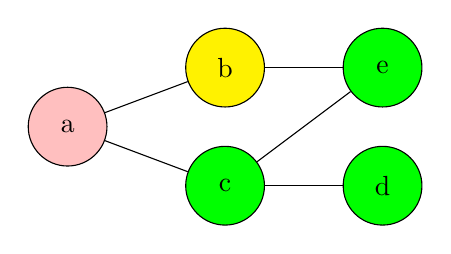
\begin{tikzpicture}[
		every node/.style={draw,circle},
		minimum size=10mm,
		node distance=2cm
	]
		\node[fill=pink] (a) at (0,0) {a};
		\node[fill=yellow] (b) at (2cm,0.75cm) {b};
		\node[fill=green] (c) at (2cm,-0.75cm) {c};
		\node[fill=green, right of=c] (d) {d};
		\node[fill=green, right of=b] (e) {e};
		\draw (a) -- (b);
		\draw (b) -- (e);
		\draw (e) -- (c);
		\draw (c) -- (d);
		\draw (a) -- (c);
	\end{tikzpicture}
	\]

	Possiamo chiederci come calcolare il valore di verità di
	\begin{center}
		Per ogni nodo $x$, se $x$ è verde allora $x$ è connesso al nodo $c$
	\end{center}
\end{frame}

\begin{frame}{Quantificatore esistenziale}
	La proposizione
	\begin{center}
		Esiste $x$ tale che bla bla blah
	\end{center}
	è vera se esiste almeno un valore che possiamo rimpiazzare in $x$ che rende vera la proposizione bla bla blah.

	Ad esempio, nel grafo di prima, la proposizione
	\begin{center}
		Esiste un nodo che non è connesso a nessun nodo verde
	\end{center}
	è falsa.
\end{frame}
\end{document}